\documentclass[runningheads]{llncs}

% ---------------------------------------------------------------
% Include basic ECCV package
 
% TODO REVIEW: Insert your submission number below by replacing '*****'
% TODO FINAL: Comment out the following line for the camera-ready version
\usepackage[review,year=2026,ID=4375]{eccv}
% TODO FINAL: Un-comment the following line for the camera-ready version
%\usepackage{eccv}

% OPTIONAL: Un-comment the following line for a version which is easier to read
% on small portrait-orientation screens (e.g., mobile phones, or beside other windows)
%\usepackage[mobile]{eccv}


% ---------------------------------------------------------------
% Other packages

% Commonly used abbreviations (\eg, \ie, \etc, \cf, \etal, etc.)
\usepackage{eccvabbrv}

% Include other packages here, before hyperref.
\usepackage{graphicx}
\usepackage{booktabs}

% The "axessiblity" package can be found at: https://ctan.org/pkg/axessibility?lang=en
\usepackage[accsupp]{axessibility}  % Improves PDF readability for those with disabilities.


% ---------------------------------------------------------------
% Hyperref package

% It is strongly recommended to use hyperref, especially for the review version.
% Please disable hyperref *only* if you encounter grave issues.
% hyperref with option pagebackref eases the reviewers' job, but should be disabled for the final version.
%
% If you comment hyperref and then uncomment it, you should delete
% main.aux before re-running LaTeX.
% (Or just hit 'q' on the first LaTeX run, let it finish, and you
%  should be clear).

% TODO FINAL: Comment out the following line for the camera-ready version
%\usepackage[pagebackref,breaklinks,colorlinks,citecolor=eccvblue]{hyperref}
% TODO FINAL: Un-comment the following line for the camera-ready version
\usepackage{hyperref}
\usepackage{adjustbox}
\usepackage[table]{xcolor} % For colors (defining darkred/darkgreen)
\usepackage{multirow} % for multi-row headers (used for "Method")
\definecolor{darkred}{rgb}{0.55, 0.0, 0.0}
\definecolor{darkgreen}{RGB}{1,50,32}

\usepackage{marvosym}
\usepackage{adjustbox}
\usepackage{graphicx}
\usepackage{amssymb}
\usepackage{pifont}
\usepackage{tabularx}
\usepackage{wrapfig}


\definecolor{darkred}{rgb}{0.6, 0, 0}
\definecolor{darkgreen}{rgb}{0, 0.6, 0}
\newcommand{\cmark}{\textcolor{darkgreen}{\ding{51}}} % Checkmark
\newcommand{\xmark}{\textcolor{darkred}{\ding{55}}} % Cross
\newcommand{\na}{\text{---}} % For N/A or unmentioned data
\usepackage[table]{xcolor}
\usepackage{colortbl}          % extra safety
\definecolor{lightblue1}{RGB}{222,235,247} % lightest blue
\definecolor{lightblue2}{RGB}{189,215,238} % medium blue
\definecolor{lightblue3}{RGB}{158,202,225} % slightly darker blue



% Support for ORCID icon
\usepackage{orcidlink}


\begin{document}

% ---------------------------------------------------------------
% TODO REVIEW: Replace with your title
\title{MODEST: Multi-Optics Depth-of-Field Stereo Dataset} 

% TODO REVIEW: If the paper title is too long for the running head, you can set
% an abbreviated paper title here. If not, comment out.
\titlerunning{}

% TODO FINAL: Replace with your author list. 
% Include the authors' OCRID for the camera-ready version, if at all possible.
\author{First Author\inst{1}\orcidlink{0000-1111-2222-3333} \and
Second Author\inst{2,3}\orcidlink{1111-2222-3333-4444} \and
Third Author\inst{3}\orcidlink{2222--3333-4444-5555}}

% TODO FINAL: Replace with an abbreviated list of authors.
\authorrunning{F.~Author et al.}
% First names are abbreviated in the running head.
% If there are more than two authors, 'et al.' is used.

% TODO FINAL: Replace with your institution list.
\institute{Princeton University, Princeton NJ 08544, USA \and
Springer Heidelberg, Tiergartenstr.~17, 69121 Heidelberg, Germany
\email{lncs@springer.com}\\
\url{http://www.springer.com/gp/computer-science/lncs} \and
ABC Institute, Rupert-Karls-University Heidelberg, Heidelberg, Germany\\
\email{\{abc,lncs\}@uni-heidelberg.de}}

\maketitle


\begin{abstract}
    Training and evaluation of state-of-the-art computer vision algorithms for reliable shallow depth of field rendering and defocus deblurring under real optical conditions remain challenging due to the constraints of lacking large-scale, full-frame resolution, high-fidelity, and real DSLR datasets. Furthermore, since shallow depth of field and defocus deblurring depend intimately on camera optical parameters, including focal length, aperture, focus plane distance, and lens geometry, models must be rigorously evaluated using high-resolution datasets with these systematic variations. We present a 5K-resolution stereo DSLR dataset, methodically varying focal length and aperture across multiple complex real scenes, capturing the optical realism and complexity of professional camera systems. The introduced dataset enables controlled analysis of geometric and optical effects for shallow depth-of-field rendering and defocus deblurring algorithms. Additionally, we provide image sets for each focal configuration, supporting classical and learning-based calibration methods. We evaluate several state-of-the-art algorithms for depth of field and defocus deblurring across focal lengths and demonstrate failure cases. By attempting to bridge the gap between synthetic data and physical camera optics, this work exposes the limitations in current state-of-the-art methods for both depth of field rendering and defocus deblurring. We release the dataset, calibration files, and evaluation code to support reproducible benchmarking and further research on real-world optical generalization.\textcolor{darkgreen}{compare with https://docs.google.com/document/d/1vsjTrOFuumkASIkkYNtputGWMiQm4qyi0jxB9T7peEY/edit?tab=t.c2uoh6o2remg}
    
    
    %Reliable Shallow Depth of Field rendering and Defocus Deburring under varying optical conditions remain significant challenges in computer vision research fields. Existing models are often bottlenecked by real-world datasets that lack high resolution, large quantity or rigorous optical metadata, limiting generalization of these models to real-world DSLR optics. In this paper, we introduce MODEST, the first high-resolution (5472×3648 px) stereo DSLR dataset designed to bridge the gap between synthetic defocus and true lens physics. The dataset contains 20000 images across 10 complex real-world scenes, captured with systematic variations in focal lengths, apertures, and stereo baseline. Unlike existing benchmarks, MODEST explicitly captures the non-linear relationship between varying apertures and focal lengths across 50 distinct optical configurations per scene. This allows analysis of geometric aberrations, bokeh morphology, and blur kernels. Each scene is filled with challenging artifacts like transparent interfaces and fine-grained textures, to stress-test SDoF rendering, defocusing, and deblurring. In addition, we provide calibration sets to calculate intrinsics and extrinsics for every configuration for disparity-guided refocusing. Our evaluation of state-of-the-art defocusing and depth-of-field models reveal significant performance degradation as focal parameters shift, highlighting the realism gap in current synthetic-heavy training regimes. We will open source the dataset and calibration suite to establish a new standard for reproducible research in high-fidelity optical modeling.
  \keywords{Depth of Field \and Stereo Imaging \and Multi-Optics Dataset}
\end{abstract}


% each section
\section{Introduction}\label{sec:intro}

% add defocus and deblurring datasets.
% number of images should be checked.

% \textcolor{green}{
% datasets in dof can be used in deblur methods as well...?
% }

\begin{table*}
\centering
\caption{Data comparison categorized for different use cases, including shallow depth-of-field rendering and defocus deblurring and deblurring. (\dag, \ddag): systematic focal length and aperture variation. RGB-P: RGB with a polarisation sensor. Active Stereo: an active stereo depth sensor. D-ToF, I-TOF: direct, indirect Time-of-Flight sensor.\vspace{-5pt}}
\label{table:dataset_comparison}
\footnotesize % Use a smaller font size for a wide table

\begin{adjustbox}{width=\textwidth}
\begin{tabular}{l c c c c c c c c c}
    \toprule
    \textbf{Dataset} & \textbf{Capture} & \textbf{Real/} & \textbf{Scene} & \textbf{Number of} & \textbf{Resolution} & \textbf{Focal Len.} & \textbf{Aperture} & \textbf{Depth} & \textbf{Calibration} \\
    & \textbf{Setup} & \textbf{Synthetic} & \textbf{Number} & \textbf{Images} & & \textbf{Variation \dag} & \textbf{Variation \ddag} & \textbf{Range} & \textbf{Set} \\
    \midrule
    \multicolumn{10}{l}{\textbf{Use Case: Shallow dof rendering and defocus deblurring}} \\
    \cmidrule{1-10}
    CUHK ('14)~\cite{Shi2014BlurDetection} & Natural Images from Internet + Binary Blur Region Masks from Human Annotators & Real & \na & 1000 & $352 \!\times\! 352$px & \na & \na & \na & \xmark \\
    RTF ('16)~\cite{d2016non} & Lytro Light‑field Camera (RGB) & Real & 22 & 44 & $360 \!\times\! 360$px & \xmark & \cmark & \na & \xmark \\
    DPDD ('19)~\cite{abuolaim2019dpdd} & Mono RGB & Real & 500 & 2000 & $1680 \!\times\! 1120$px & \xmark & \xmark & $0.3\text{m} - 10\text{m}$ & \xmark \\
    LFDOF ('21)~\cite{ruan2021aifnet} & Light-field Camera + LiDAR & Real & \na & 23978 & $375 \!\times\! 540$px & \xmark & \xmark & $0.3\text{m} - 10\text{m}$ & \xmark \\
    RealDOF ('21)~\cite{lee2021iterative} & Dual-camera with a beam splitter (RGB) & Real & 50 & 100 & $1536 \!\times\! 2320$px & \xmark & \cmark & \na & \xmark \\
    BLB ('22)~\cite{zheng2022blur} & Synthetic renderings from Blender & Synthetic & 10 & 1000 & $1920 \!\times\! 1080$px & \xmark & \cmark & $0.5\text{m} - 10\text{m}$ & \xmark \\
    VABD ('24)~\cite{huang2024vabd} & Mono RGB & Real & 535 & 2940 & $1536 \!\times\! 1024$px & \xmark & \cmark & \na & \xmark \\
    RealBokeh ('25)~\cite{seizinger2025bokehlicious} & Mono RGB (Canon EOS R6 II) & Real & 300 & 23000 & $6000 \!\times\! 4000$px & \cmark & \cmark & \na & \xmark \\
    MODEST (Ours) & Stereo RGB (Canon 6D) & Real & 9 & 20000 & $\mathbf{5472 \!\times\! 3648}$px & \cmark & \cmark & $0.5\text{m} - 10\text{m}$ & \cmark \\
    \midrule
    \multicolumn{10}{l}{\textbf{Use Case: Deblurring}} \\
    \cmidrule{1-10}
    GoPro ('17)~\cite{nah2017deep} & GoPro Hero4 Black Camera & Synthetic & 33 & 3214 & $1280 \!\times\! 720$px & \xmark & \xmark & \na & \xmark \\
    DeepLens ('18)~\cite{lijun2018deeplens} & Dual-lens Camera + Thin-lens model and Billboards & Real + Synthetic & \na & 502462 & $3024 \!\times\! 4032$px & \xmark & \cmark & \na & \xmark \\
    HIDE ('19)~\cite{shen2019human} & Gopro Hero4 Black Camera & Synthetic & 31 & 16844 & $1280 \!\times\! 720$px & \xmark & \xmark & $0\text{m} - 3\text{m}$ & \xmark \\
    REDS ('19)~\cite{nah2019ntire} & GoPro Hero6 Black Camera & Synthetic & 300 & 30000 & $1280 \!\times\! 720$px & \xmark & \xmark & $0\text{m} - 3\text{m}$ & \xmark \\
    SYNDOF ('19)~\cite{lee2019deep} & Thin-lens model & Synthetic & \na & 8231 & (960-2000) $\!\times\!$ (436-2000)px & \cmark & \cmark & $0.5\text{m} - 80\text{m}$ & \xmark \\
    RealBlur ('20)~\cite{rim2020real} & Dual-camera System with a Beam Splitter & Real & 232 & 18952 & $680 \!\times\! 772$px & \xmark & \xmark & \na & \cmark \\
    BSD-B ('20)~\cite{Chen_2020_CVPR} & Convolving Sharp Images with Uniform Disk Kernels & Synthetic & 500 & 40000 & (320-480) $\!\times\!$ (320-480)px & \na & \cmark & \na & \na \\
    NTIRE ('21)~\cite{nah2021ntire} & GoPro Hero6 Black Camera & Synthetic & 300 & 30000 & $1280 \!\times\! 720$px & \xmark & \xmark & $0.5\text{m} - infinity$ & \xmark \\
    RSBlur ('22)~\cite{rim2022realistic} & Dual-camera system & Real & 697 & 13358 & $1920 \!\times\! 1200$px & \xmark & \xmark & $1\text{m} - infinity$ & \xmark \\
    iDFD ('23)~\cite{nazir2023idfd} & Dual-sensor Rig (RGB) + Microsoft Kinect (Depth) & Real & \na & 1528 & $1050 \!\times\! 1050$px & \xmark & \cmark & $0\text{m} - 10\text{m}$ & \xmark \\
    GS-Blur ('24)~\cite{lee2024gs} & 3D Gaussian Splatting Model & Synthetic & 18542 & 312418 & $1280 \!\times\! 720$px & \cmark & \xmark & \na & \xmark \\
    QPDD ('25)~\cite{chen2025quad} & 50-megapixel Quad-Pixel Sensor & Real & 300 & 9870 & (1080-4096) $\!\times\!$ (1280-3072)px & \xmark & \cmark & $0.2\text{m} - infinity$ & \xmark \\
    MODEST (Ours) & Stereo RGB (Canon 6D) & Real & 9 & 20000 & $\mathbf{5472 \!\times\! 3648}$px & \cmark & \cmark & $0.5\text{m} - 10\text{m}$ & \cmark \\
    %\midrule
    %\multicolumn{10}{l}{\textbf{Use Case: Optical illusions}} \\
    %\cmidrule{1-10}
    %3D-Visual-Illusion ('25)~\cite{yao20253d} & Stereo RGB + LiDAR & Real + Synthetic & 3000 & \na & $1080 \!\times\! 1920$px & \na & \na & $0.5\text{m}-50\text{m}$ & \xmark \\
    %MonoTrap ('25)~\cite{bartolomei2025stereo} & Stereo Image RGB + LiDAR & Real & 26 & \na & $585 \!\times\! 375$px & \xmark & \xmark & $0\text{m} - 10\text{m}$ & \xmark \\
    %MODEST (Ours) & Stereo RGB (Canon 6D) & Real & 9 & 20000 & $\mathbf{5472 \!\times\! 3648}$px & \cmark & \cmark & $0.5\text{m} - 10\text{m}$ & \cmark \\
    \bottomrule
\end{tabular}
\end{adjustbox}
\vspace{-6pt}
\end{table*}

% Depth estimation is a fundamental and essential application of computer vision, with applications including robotics, autonomous vehicles, augmented or mixed reality, 3D scene creation and novel view synthesis, among others. Recent years have been revolutionary in creating high-quality and precise depth maps and 3D scenes with breakthrough deep-learning models such as FoundationStereo~\cite{wen2025stereo} and Depth Anything~\cite{yang2024depth} for depth estimation and neural radiance fields (NeRFs)~\cite{mildenhall2020nerfrepresentingscenesneural} and Gaussian splatting (GS)~\cite{kerbl20233dgaussiansplattingrealtime} for 3D scene reconstruction.

%Shallow depth of field (DoF) rendering and defocus deblurring are two essential applications in computer vision. Shallow DoF renders a narrow focal plane sharp while blurring foreground and background, making it useful as a preprocessing step for salient object detection and scene segmentation. Shallow DoF could be also used for depth estimation that approximates the distance between objects and a camera. Unlike DoF, defocus deblurring is to restore blurred regions caused by a lens being out of focus. A classical application for defocus deblurring is information recovery where deblurring algorithms recover high-frequency details (e.g., sharp edges). With shallow DoF and defocus deblurring operations, it is easy to mimic real-world optics in all-focused digital images.

Shallow depth of field (DoF) rendering is the process of mimicking the optical blur that occurs in a physical camera with a wide aperture. The effect of shallow DoF is to guide viewers to only focus on a narrow, sharp region of the image with a blurred background and foreground. With synthetically mimicked optical blur, in a study of human-computer interaction (HCI)~\cite{hillaire2008using}, shallow DoF rendering could serve as a perceptual-attentive cue where, by blurring non-important information, the brain can process the sharp area quickly. In addition, shallow DoF rendering is a technique for improving depth from defocus algorithms ~\cite{suwajanakorn2015depth}.


%Notably, the applications of depth estimation and single- or multi-view synthesis for computer vision tasks have been studied, and there are popular datasets for model evaluation; however, existing datasets tend to have relatively low-resolution RGB images (e.g., NYU Depth V2~\cite{silberman2012nyu}, TUM RGB-D~\cite{sturm2012tum}, or VOID~\cite{wang2020void} or lack systematic variations of focal lengths and aperture settings (e.g., ScanNet++~\cite{yeshwanth2024scannetpp}, Replica~\cite{straub2019replica} , or HAMMER~\cite{laga2022hammer}. Another limitation of the existing datasets is that the scene complexity is relatively low, i.e., there are only a few scenes that contain small objects (e.g., flowers and leaves), optical illusions, and reflective and transparent surfaces (e.g., glass doors).

%Notably, training and evaluation for shallow DoF and defocus deblurring algorithms remain constrained by the lack of large-scale, full-frame resolution, high-fidelity, real DSLR datasets, limiting real-world generalization and evaluation of models trained on synthetic or low-resolution data. Shallow DoF and defocus deblurring are governed by focal length, aperture, and focus distance. Meaningful evaluation therefore requires datasets that systematically vary these parameters at high resolution, a condition no existing benchmark satisfies. Modern camera systems in augmented reality (AR/VR), autonomous vehicles or robots are equipped with stereo or multiple camera systems, where models trained on monocular datasets cannot exploit stereo disparity and may underperform.

In contrast to DoF, defocus deblurring is a process that utilizes image sharpening algorithms to restore high-frequency information lost in blurred regions caused by a lens being out of focus. Due to this, defocus deblurring is compelling to computer vision applications, including autonomous driving and robotics~\cite{shah2025impact} and surveillance and security~\cite{hillaire2008using}. For autonomous driving and robotics, deblurring algorithms ensure sharp regions for safety navigation. Defocus deblurring algorithms are used in forensic analysis to reconstruct sharpened regions given blurred images.


%Calibration algorithms continue seeing advanced. To recalculate calibration parameters through newer algorithms, we need access to high-resolution, multi-view calibration images, which are absent in many public datasets in Table~\ref{table:dataset_comparison}. Compared with many existing datasets, we provide a global intrinsics calibration set and per-focal-length extrinsic calibration sets, allowing recalibration flexibility.

Reliable shallow DoF rendering and defocus deblurring under real optical conditions remain challenging for state-of-the-art DoF and defocus deblurring models due to the lack of large-scale, full-frame resolution, high-fidelity, real DSLR datasets. Table \ref{table:dataset_comparison} shows dataset comparisons among different datasets. Most early datasets contain large numbers of scenes from indoor and outdoor environments; however, these datasets encounter several limitations, including low-resolution images and the lack of systematic variations of focal length and apertures. DPDD~\cite{abuolaim2019dpdd} is a recent 6K-resolution dataset for model training and evaluation in defocus deblurring, but this dataset does not systematically cover a varying range of focal lengths and apertures. QPDD~\cite{chen2025quad} is another defocus deblurring dataset captured by a camera with sub-aperture views, allowing models to use these sub-aperture views to deblur a pixel. The limitation of the sub-aperture views is the micro-parallax problem, where it is difficult to distinguish between actual depth and sensor noise due to the tiny physical distance between the sub-pixels. Additionally, the existing datasets do not provide calibration sets for recalculating calibration parameters through newer algorithms. Thus, we provide a global intrinsic calibration set and per-focal-length extrinsic calibration sets, allowing recalibration flexibility.

%Further, calibration algorithms continue seeing advancement. To recalculate calibration parameters using newer algorithms, we need access to high-resolution, multi-view calibration images, which are absent in many public datasets (Table~\ref{table:dataset_comparison}). We provide a global intrinsics calibration set and per-focal-length extrinsic calibration sets, allowing recalibration flexibility. 


\subsection{Contributions}\label{subsec:contribution}

%MODEST addresses three gaps simultaneously: high resolution, stereo geometry, and systematic optical variation where none of which existing datasets provide together. Our proposed dataset, Multi-Optics Depth-of-Field Stereo Dataset (MODEST), contains 20000 images across 10 scenes at high resolution (5472 $\times$ 3648 px). Each scene has 10 focal lengths and 5 apertures per focal length, with a dedicated calibration image set per focal length consisting of large checkerboard images (see Table~\ref{table:dataset_comparison}). The dataset also includes challenging visual elements such as optical illusions, reflective surfaces, ambiguous background depths, sharp brightness changes, etc. 

%Our second contribution is that we implement and evaluate state-of-the-art monocular and stereo depth estimation, shallow depth-of-field, and deblurring methods on our dataset. We also produce systematic performance evaluation for shallow depth-of-field and deblurring methods across focal lengths and highlight the need to train and test these models on datasets such as ours, which offer explicit, wide coverage of camera optics.

%We open source the dataset, illustrations and visuals, processing and evaluation tools to push research frontiers for purely non-commercial and academic purposes.

In this paper, we introduce the first high-resolution stereo DSLR dataset called the Multi-Optics Depth-of-Field Stereo Dataset (MODEST), capturing methodical variations of focal length and aperture across 10 complex real scenes and the optical realism and complexity of professional camera systems. The MODEST dataset addresses three major limitations, high resolution, stereo geometry, and systematic optical variation, in existing datasets. Our MODEST dataset contains 20000 images across 10 scenes at high resolution (5472 $\times$ 3648 px). Each scene has 10 focal lengths and 5 apertures per focal length, with a dedicated calibration image set per focal length consisting of large checkerboard images (see Table~\ref{table:dataset_comparison}). Therefore, we can recalculate calibration parameters through newer calibration algorithms by accessing high-resolution and multi-view calibration images. The dataset also includes challenging visual elements such as optical illusions, reflective surfaces, ambiguous background depths, and sharp brightness changes.

The second contribution of this paper is that we perform a systematic analysis of state-of-the-art DoF and defocus deblurring models on our proposed dataset across varying focal lengths. With these performance analysis results, this paper reveals the limitations in current state-of-the-art models for both depth of field rendering and defocus deblurring.

The final contribution is that we release our MODEST dataset, illustrations, and visuals, processing and evaluation tools to push research frontiers for purely non-commercial and academic purposes.





\subsection{Related Datasets}\label{subsec:related_datasets}

% add one small paragraph to be a summary.
In this subsection, we will briefly introduce and discuss related existing datasets for depth of field and defocus deblurring as mentioned in 
Table~\ref{table:dataset_comparison}

% Shallow depth-of-field rendering

Shallow depth-of-field (DoF) rendering is a process of synthetically creating the photographic effect where only a small portion of the scene in images is in focus, while the rest is blurred. The idea of shallow DoF is to mimic the optics of real cameras with wide apertures. The CUHK~\cite{Shi2014BlurDetection} dataset is the earliest data for DoF applications, but this dataset does not have variations of focal lengths and apertures for the collected images because they are collected from Internet. DPDD~\cite{abuolaim2019dpdd} is a pioneering dataset for shallow DoF rendering; however, the limitations of the DPDD~\cite{abuolaim2019dpdd} dataset include one camera model and optics setup, and only one blur condition. EBB!~\cite{ignatov2020rendering} is another dataset for shallow DoF rendering, but is no longer accessible. Recent data sets for shallow DoF rendering are BLB~\cite{zheng2022blur} and VABD~\cite{huang2024vabd}. Both datasets solve the issue of single optics and one blur condition in DPDD~\cite{abuolaim2019dpdd} by providing either multiple blur levels per scene or capturing multiple apertures per scene. The problems with the BLB and VABD dataset are that it only provides multiple blur levels or calibration parameters. The most recent dataset for DoF is RealBokeh~\cite{seizinger2025bokehlicious}.While it captures high-resolution RGB images with both focal length and aperture variation across a large number of scenes, it remains monocular and provides no calibration sets, making recalibration or adaptation to new lens configurations impossible. Furthermore, as RealBokeh prioritizes scene diversity over per-scene optical coverage, it does not capture the same scene across a systematic grid of focal length and aperture combinations, making it difficult to disentangle blur caused by aperture width from blur caused by subject distance. MODEST addresses all three of these limitations through stereo capture, per-focal-length calibration sets, and a controlled 50-configuration grid per scene.

% DoF capture setting discussion.
%Varying focal lengths, focal distances, and apertures are essential optical properties for DoF images. To capture images with variations in focal lengths, distances, and apertures, a light-field camera records the spatial location and angular directions of incoming light rays. Therefore, the light-field camera easily captures varied apertures. The images in both RTF~\cite{d2016non} and LFDOF~\cite{ruan2021aifnet} datasets are collected by a light-field camera. RTF contains images captured by physical aperture variations, but LFDOF is captured with a fixed camera aperture. Additionally, for both datasets, the captured images are low resolution due to the nature of the light-field camera. Unlike RTF and LFDOF, RealDOF~\cite{lee2021iterative} is captured by a dual-camera sensor that simulates shallow DoF by retaining sharp subjects in focus and blurring the background; however, the limitation of the dual-camera is having a small baseline between the two cameras, and it cannot reproduce true optical DoF.

% DoF capture setting discussion.
To capture DoF images with variations in focal lengths, distances, and apertures, a light-field camera records the spatial location and angular directions of incoming light rays. Therefore, the light-field camera easily captures varied apertures. The images in both RTF~\cite{d2016non} and LFDOF~\cite{ruan2021aifnet} datasets are collected by a light-field camera. RTF contains images captured by physical aperture variations, but LFDOF is captured with a fixed camera aperture. Additionally, for both datasets, the captured images are low resolution due to the nature of the light-field camera. Unlike RTF and LFDOF, RealDOF~\cite{lee2021iterative} is captured by a dual-camera sensor that simulates shallow DoF by retaining sharp subjects in focus and blurring the background; however, a dual-camera has a small baseline between the two cameras and cannot reproduce true optical DoF.


% defocus deblurring
%To yield defocus or blurred images, a GoPro black camera is used to synthesize blurred images through averaging consecutive frames in a high-speed video for the GoPro~\cite{nah2017deep}, HIDE~\cite{shen2019human}, REDS~\cite{nah2019ntire}, NTIRE~\cite{nah2021ntire} dataset. The constraint of the blurred images captured by either a Hero4 or Hero6 camera is fixed defocus, which fails to defocus distant objects. Therefore, the GoPro camera is incapable of creating “bokeh” (background defocus) for any object further than a few inches away. For the DeepLens~\cite{lijun2018deeplens}, RealBlur~\cite{rim2020real}, and iDFD~\cite{nazir2023idfd} datasets, they create blurred images through stereo disparity, which is a baseline between a wide-angle lens and a telephoto lens camera, created by a dual-lens camera. Then, it applies the disparity map to compute pixel-wise blurriness levels for foreground and background in the image. Due to the disparity map, the constraints of the dual-lens camera contain boundary confusion and depth Discontinuity. Unlike previous defocus and blurring datasets, GS-Blur~\cite{lee2024gs} applies a 3D Gaussian Splatting model to synthesize blurred images. The major bottleneck of the blurred images is low-frequency bias, where the images lose detail because of over-smoothing. The QPDD~\cite{chen2025quad} dataset contains blurred images captured by a quad-pixel sensor that captures defocus information by splitting the light that enters a single microlens into four different sub-aperture views; however, the blurred images captured by the quad-pixel sensor are still yielded by fixed apertures.

In defocus deblurring, a GoPro black camera is used to synthesize blurred images through averaging consecutive frames in a high-speed video for the GoPro~\cite{nah2017deep}, HIDE~\cite{shen2019human}, REDS~\cite{nah2019ntire}, NTIRE~\cite{nah2021ntire} dataset. The constraint of the blurred images captured by either a Hero4 or Hero6 camera is fixed defocus, which fails to defocus distant objects. Therefore, the GoPro camera is incapable of creating “bokeh” (background defocus) for any object further than a few inches away. For the DeepLens~\cite{lijun2018deeplens}, RealBlur~\cite{rim2020real}, and iDFD~\cite{nazir2023idfd} datasets, they create blurred images through stereo disparity, which is a baseline between a wide-angle lens and a telephoto lens camera, created by a dual-lens camera. Then, it applies the disparity map to compute pixel-wise blurriness levels for foreground and background in the image. Due to the disparity map, the constraints of the dual-lens camera contain boundary confusion and depth Discontinuity. Unlike previous defocus and blurring datasets, GS-Blur~\cite{lee2024gs} applies a 3D Gaussian Splatting model to synthesize blurred images. The major bottleneck of the blurred images is low-frequency bias, where the images lose detail due to over-smoothing. The QPDD~\cite{chen2025quad} dataset contains blurred images captured by a quad-pixel sensor that captures defocus information by splitting the light that enters a single microlens into four different sub-aperture views; however, the blurred images captured by the quad-pixel sensor are difficult to distinguish between actual depth and sensor noise due to the tiny physical distance between the sub-pixels.


% Optical illusions
%Optical illusions in depth-model evaluation refer to probing the limitations of depth-estimation models via perceptual tricks or visually deceptive scenes. These illusions reveal where a model relies on texture, shading, or priors in the images rather than true geometric reasoning. 3D-Visual-Illusion~\cite{yao20253d} is a dataset for optical illusion, and it has been used for human vision experiments where illusions help understand how the human visual system infers 3D structure rather than directly measuring it. The limitation of this dataset is the lack of calibration sets for image calibration. The MonoTrap~\cite{bartolomei2025stereo} is a recent dataset for optical illusions; however, this data only has low-resolution images for the optical illusion task. Thus, many optical illusions in the real world (e.g., heat haze or subtle glass reflection) are missing in low-resolution images. Additionally, the optical illusion images are captured at a fixed number of apertures. This causes MonoTrap to be incapable of mimicking how real professional cameras operate.

% ours (MODEST)
Compared to existing datasets, our proposed MODEST dataset includes both high-resolution stereo RGB images captured with different focal lengths and aperture settings per scene, along with calibration sets provided for calibration algorithms. They enable recalibration or adaptation to lens drift or new alignment while performing camera calibration. With high-resolution images (i.e., 5K-resolution images), the MODEST enables captured images to preserve much detail for optical illusions. This allows researchers to analyze a model’s illusion errors comprehensively and mimic the operations of professional cameras in optical illusions. Additionally, the benefit of our MODEST dataset for shallow DoF rendering tasks is that it contains physical defocused and sharp images (i.e., ground truth) due to its wide range of apertures. In addition, compared to the RealBokeh dataset, MODEST captures the same scene across a mixture of 50 different optical configurations. This allows researchers to assess the model’s quantitative results through high-scene varieties. As we showed with experiments, the Bokehlicious model trained on the RealBokeh dataset is tuned on a particular lens and performs slightly worse on the lens of this dataset. Our MODEST dataset thus offers a second lens datapoint with similar high-resolution images for a slightly more generalizability test.



% stereo dataset + multi-vieew stereo dataset --> move it to supplumentary material
%Early datasets for depth-model evaluation, including KITTI~\cite{geiger2012kitti, Menze2015ISA}, NYU Depth V2~\cite{silberman2012nyu} , ScanNet~\cite{dai2017scannet}, TUM RGB-D~\cite{sturm2012tum}, and iBims-1~\cite{koch2018evaluation}, contain low-resolution RGB and depth images. Due to low resolutions, small objects and detailed context in RGB and depth images are difficult to recognize and evaluate. Most recently, new datasets, including DIML outdoor~\cite{wong2020diml}, HAMMER~\cite{laga2022hammer},and ScanNet++~\cite{yeshwanth2024scannetpp}, with high-resolution RGB and depth images, were proposed to be adapted to depth-model evaluation problems. The limitation of this data set is that sensors with constant focal lengths and aperture settings are used to capture RGB frames. Thus, the captured scenes are not varied enough for depth estimation evaluation. The Middlebury14~\cite{Scharstein_2014_High_Resolution_Stereo} and Middlebury21~\cite{Scharstein2002taxonomy} datasets include high-resolution stereo RGB images, so they have been used for stereo matching and disparity estimation; however, these stereo RGB images are captured by the image sensors with constant focal lengths and apertures. The HAMMER~\cite{laga2022hammer} and ScanNet++~\cite{yeshwanth2024scannetpp} also include high-resolution RGB and depth images, but they are also captured by imaging sensors with constant focal lengths and apertures. Regardless of the above datasets, multi-view stereo datasets have been made available. ETH3D~\cite{schops2017eth3d} and DDAD~\cite{garg2020ddad} datasets comprise images acquired under varying lighting conditions. The limitation of multi-view stereo datasets is variations in focal lengths and apertures during the data acquisition process. 

% 3D scence reconstruction.  --> move it to supplumentary material
%3D scene reconstruction is another fundamental task in computer vision studies, and pioneering datasets, such as Sintel~\cite{butler2012sintel}  and DIODE ~\cite{vlasic2019diode}, are made available. Sintel~\cite{butler2012sintel} is a synthetic dataset made through synthetic renderings from the 3D film Sintel. Due to the synthetic images, the color distribution of the scenes in the Sintel~\cite{butler2012sintel} dataset differs from real scenes captured by real sensors ~\cite{jia2025secret}. DIODE~\cite{vlasic2019diode} is another public dataset used for 3D reconstruction tasks. The scenes have varying illumination changes due to indoor and outdoor environments. The problem with the DIODE~\cite{vlasic2019diode} dataset is that calibration sets (i.e., calibration images) are not provided. Therefore, the calibration parameters are difficult to reuse to calibrate captured images from new sensors.








%\begin{table*}
%\centering
%\caption{Data comparison categorized per use-case. This table focuses on stereo dataset, multi-view stereo, and 3D scene reconstruction. (\dag, \ddag): systematic focal length and aperture variation. RGB-P: RGB with polarisation sensor. Active Stereo: an active stereo depth sensor. D-ToF, I-TOF: direct, indirect Time-of-Flight sensor.\vspace{-5pt}}
%\label{table:dataset_comparison}
%\footnotesize % Use a smaller font size for a wide table

%\begin{adjustbox}{width=\textwidth}
%\begin{tabular}{l c c c c c c c c c}
%    \toprule
%    \textbf{Dataset} & \textbf{Capture} & \textbf{Real/} & \textbf{Scene} & \textbf{Number of} & \textbf{Resolution} & \textbf{Focal Len.} & \textbf{Aperture} & \textbf{Depth} & \textbf{Calibration} \\
%    & \textbf{Setup} & \textbf{Synthetic} & \textbf{Number} & \textbf{Images} & & \textbf{Variation \dag} & \textbf{Variation \ddag} & \textbf{Range} & \textbf{Set} \\
%    \midrule
%    \multicolumn{10}{l}{\textbf{Use Case: Stereo Dataset and Depth-model Evaluation}} \\
%    \cmidrule{1-10} % Partial rule to separate section title from data
%    KITTI ('12)~\cite{geiger2012kitti} & Stereo RGB + LiDAR & Real & 389 & 389 & $1242 \!\times\! 375$px & \xmark & \xmark  & $0.5\text{m} - 80\text{m}$ & \xmark \\
%    NYU Depth V2 ('12)~\cite{silberman2012nyu} & Mono RGB-D (Kinect v1) & Real & 464 & \na & $640 \!\times\! 480$px & \xmark & \xmark & $0.5\text{m} - 10\text{m}$ & \xmark \\
%    TUM RGB-D ('12)~\cite{sturm2012tum} & Mono RGB-D (Kinect v1) & Real & 39 & \na & $640 \!\times\! 480$px & \xmark & \xmark & $0.5\text{m} - 5\text{m}$ & \xmark \\
%    Middlebury14 ('14)~\cite{Scharstein_2014_High_Resolution_Stereo} & Stereo Image RGB + high-precision structured-light scanning & Real & 38 & 31 & $3000 \!\times\! 2000$px & \xmark & \xmark & $0.3\text{m} - 10\text{m}$ & \xmark \\
%    KITTI ('15)~\cite{Menze2015ISA} & Stereo Image RGB + LiDAR & Real & 400 & 400 & $1242 \!\times\! 375$px & \xmark & \xmark & $0\text{m} - 120\text{m}$ & \xmark \\
%    vKITTI ('16)~\cite{gaidon2016vkitti} & Virtual stereo cameras (Unity) & Synthetic & 5 & 21260 & $1242 \!\times\! 375$px & \xmark & \xmark & $0.5\text{m} - 100\text{m}$ & \xmark \\
%    ScanNet ('17)~\cite{dai2017scannet} & Mono RGB-D (iPad + PrimeSense) & Real & 1513 & \na & (640-1296) $\!\times\!$ (480-968)px & \xmark & \xmark & $0.2\text{m} - 10\text{m}$ & \xmark \\
%    Matterport3 ('17)~\cite{chang2017matterport3d} & Multi-camera (360-degree RGB-D) & Real & 90 & \na & $1280 \!\times\! 1024$px & \xmark & \xmark & $0.2\text{m} - 20\text{m}$ & \xmark \\
%    iBims-1 ('18)~\cite{koch2020ibims1} & Mono RGB (DSLR) & Real & 100 & \na & (640-1500) $\!\times\!$ (480-1000)px & \xmark & \xmark & $0.5\text{m} - 10\text{m}$ & \xmark \\
%    VOID ('20)~\cite{wang2020void} & Mono RGB-D (RealSense D435i) & Real & 52 & \na & $640 \!\times\! 480$px & \cmark & \xmark & $50\text{m}$ & \xmark \\
%    DIML outdoor ('20)~\cite{wong2020diml} & Stereo RGB (ZED camera) & Real & 132 & 132 & $1920 \!\times\! 1080$px & \xmark & \xmark & $0.5\text{m} - 100\text{m}$ & \xmark \\
%    Middlebury21 ('21)~\cite{Scharstein2002taxonomy} & Stereo Image RGB (handheld mobile) + high-precision structured-light scanning & Real & 24 & 24 & $4032 \!\times\! 3024$px & \xmark & \xmark & $0.3\text{m} - 10\text{m}$ & \xmark \\
%    HAMMER ('22)~\cite{laga2022hammer} & Multi-camera (RGB-P + Active/D/I-ToF) & Real & 13 & \na & $1280 \!\times\! 720$px & \xmark & \xmark & $10\text{m}$ & \xmark \\
%    ScanNet++ ('24)~\cite{yeshwanth2024scannetpp} & Mono RGB-D (iPad + Structure Sensor) & Real & 380 & \na & $1920 \!\times\! 1440$px & \xmark & \xmark & $0.2\text{m} - 20\text{m}$ & \xmark \\
%    MODEST (Ours) & Stereo RGB (Canon 6D) & Real & 9 & 20000 & $\mathbf{5472 \!\times\! 3648}$px & \cmark & \cmark & $0.5\text{m} - 10\text{m}$ & \cmark \\
%    \midrule % Separator for main sections
%    \multicolumn{10}{l}{\textbf{Use Case: Multi-view Stereo}} \\
%    \cmidrule{1-10}
%    ETH3D ('17)~\cite{schops2017eth3d} & Multi-camera (DSLR + LiDAR + Stereo) & Real & 25 & 47 & $2048 \!\times\! 1536$px & \xmark & \xmark & $0.5\text{m} - 50\text{m}$ & \xmark \\
%    ETH3D low-res 2-view (17')~\cite{schops2017multi} & Stereo Image RGB + Multi-view Stereo & Real & 40 & 47 & $752 \!\times\! 480$px & \xmark & \xmark & $1\text{m} - 30\text{m}$ & \cmark \\    
%    Replica ('19)~\cite{straub2019replica} & Mono RGB (DSLR + LiDAR) & Synthetic & 18 & \na & $1080 \!\times\! 1080$px & \xmark & \xmark & $0.1\text{m} - 10\text{m}$ & \xmark \\
%    DDAD ('20)~\cite{garg2020ddad} & Multi-camera (shutter + LiDAR) & Real & 200 & \na & $1600 \!\times\! 900$px & \xmark & \xmark & $0.5\text{m} - 100\text{m}$ & \xmark \\
%    MODEST (Ours) & Stereo RGB (Canon 6D) & Real & 9 & 20000 & $\mathbf{5472 \!\times\! 3648}$px & \cmark & \cmark & $0.5\text{m} - 10\text{m}$ & \cmark \\
%    \midrule
%    \multicolumn{10}{l}{\textbf{Use Case: 3D static and dynamic scene generation}} \\
%    \cmidrule{1-10}
%    Sintel ('12)~\cite{butler2012sintel} & Synthetic renderings from 3D film & Synthetic & 23 & \na & $1024 \!\times\! 436$px & \xmark & \xmark & $0\text{m} - 80\text{m}$ & \xmark \\
%    DIODE ('19)~\cite{vlasic2019diode} & Mono RGB-D (FARO Focus S350) & Real & 30 & \na & $1024 \!\times\! 768$px & \xmark & \xmark & $0.5\text{m} - 350\text{m}$ & \xmark \\
%    MODEST (Ours) & Stereo RGB (Canon 6D) & Real & 9 & 20000 & $\mathbf{5472 \!\times\! 3648}$px & \cmark & \cmark & $0.5\text{m} - 10\text{m}$ & \cmark \\
    
%    \bottomrule
%\end{tabular}
%\end{adjustbox}
%\vspace{-6pt}
%\end{table*}



\section{Data Acquisition and Processing}\label{sec:method}
The following sections give details on data collection, calibration process and optical illusions in this dataset, and multiple use-cases. 

\begin{figure*}[h]  % * makes it span both columns
    \centering
% calibration illustration.
% \begin{wrapfigure}{1\textwidth}
%     \centering
    \includegraphics[width=\textwidth]{imgs/calib+cam+refl+detl.pdf}
    \caption{Data acquisition and scene categories. We utilize a stereo camera assembly and diverse calibration viewpoints to capture objects with complex optical properties, such as reflective surfaces and fine details and 3D textures.}
    \label{fig:cal_illustration}
\end{figure*}


\subsection{Camera setup and configuration}\label{subsec:cal_illustration}

The camera assembly consists of two \textit{Canon EOS 6D} full-frame DSLR cameras mounted in a synchronized stereo configuration with identical lens setups as seen in Figure~\ref{fig:cal_illustration} under "Stereo Camera Assembly". Each camera is equipped with a 28–70\,mm zoom lens, enabling controlled variation of focal length. The system supports a wide aperture range from F22 to F2.8, allowing independent adjustment to systematically capture scenes with varying depth-of-field and blur characteristics. To ensure alignment between the stereo pair, remote shutter triggering is used to achieve synchronous image capture, preventing motion inconsistencies between the two views. The cameras are mounted on a balanced, height-adjustable tripod rig that allows precise control over the stereo baseline distance. This adjustable baseline upto a max of 30 cm enables flexible capture configurations suitable for different scene scales while maintaining geometric consistency.


\subsection{Data Design and Calibration}\label{subsec:data_design}

% \begin{figure*}[h]  % * makes it span both columns
%     \centering
% % calibration illustration.
% % \begin{wrapfigure}{1\textwidth}
% %     \centering
%     \includegraphics[width=\textwidth]{imgs/calib+cam+refl+detl.pdf}
%     \caption{Data acquisition and scene categories. We utilize a stereo camera assembly and diverse calibration viewpoints to capture objects with complex optical properties, such as reflective surfaces and fine details and 3D textures.}
%     \label{fig:cal_illustration}
% \end{figure*}

% \begin{figure}
%     \centering
%     \includegraphics[scale=0.9]{imgs/calib+cam+refl+detl.png}
%     \caption{ADD CAPTION}
%     \label{fig:cal_illustration}
% \end{figure}
During data collection and the calibration process, we captured 10 distinct scenes using a balanced stereo setup composed of two identical Canon EOS 6D cameras and lenses capturing full-frame images. For each scene, we acquired image sets across 10 different focal lengths: \{28, 32, 36, 40, 45, 50, 55, 60, 65, and 70\}mm to examine how focal variation influences geometric accuracy and depth reconstruction. Each focal length yields approximately 100 stereo image pairs: 20 pairs per aperture across five aperture settings (f/2.8, f/4, f/5.6, f/11, f/22).

The calibration set, captured using a fixed aperture, consists of approximately 100 stereo image pairs (left and right) acquired from multiple viewpoints to ensure robust and accurate geometric calibration (Figure~\ref{fig:cal_illustration}) as visualized under "calibration viewpoints”. These images are used to estimate the intrinsic and extrinsic parameters required for accurately calibrated images used for shallow DoF and defocus deblurring use cases.



\subsection{Scene Diversity and Visual Complexity}\label{subsec:data_illu}

\begin{table}[t]
\centering
\caption{Types of scene objects included to capture diverse visual and optical properties.}
\label{tab:scene_objects}
\small 
\begin{tabularx}{\linewidth}{>{\raggedright\arraybackslash}p{3cm} X} 
\toprule
\textbf{Category} & \textbf{Examples of Objects} \\
\midrule
\textbf{Reflective surfaces} & Reflective spheres, ceramic jars, transparent containers, semi-transparent doors \\ %& Mirrors, reflective spheres, metallic balls, reflective cubes, films, crystal spheres, balloons, glass jars, transparent containers, golden foils. \\
\addlinespace[0.6em]
\textbf{Fine Details} & Small toys, geometric props, stacked objects, patterned surfaces, small structural shapes, flowers, textured objects, shaped lights. \\ %, torch. \\
%\addlinespace[0.6em]
%\textbf{Optical Illusions} & Printed illusion patterns, structured geometric illusion prints, target prints. \\  %& Printed illusion patterns, checkerboard targets, structured geometric illusion prints, target prints. \\
\bottomrule
\end{tabularx}
\end{table}

%The dataset contains ten scenes as illustrated in Figure~\ref{fig:data} designed to capture diverse visual and optical properties, summarized in Table~\ref{tab:scene_objects} and showed some examples in Figure~\ref{fig:cal_illustration} under "Reflective Surfaces" and "Fine Details 3D Textures". Scene 1 represents the most complex configuration and is intentionally designed to be highly challenging for  MVS, defocus, and deblurring tasks. It contains closely arranged objects including reflective materials, decorative elements, lamps, and light-emitting sources, along with flowers containing thin petals and stems. These objects are densely arranged to create occlusions and complex depth boundaries, while a large banner is placed as the background. Scene 2 presents a simpler tabletop setting with a closed window as the background and primarily focuses on optical illusion patterns mixed with scattered toys.

The MODEST dataset comprises 10 scenes as illustrated in Figure~\ref{fig:data}, designed to capture diverse visual and optical properties, summarized in Table~\ref{tab:scene_objects}. Figure~\ref{fig:cal_illustration} under "Reflective Surfaces" and "Fine Details 3D Textures” shows some example images with a variety of scene objects. Scene 1 represents the most complex configuration and is intentionally designed to be highly challenging for DoF, defocus, and deblurring tasks. This scene has closely arranged objects, including reflective materials, decorative elements, lamps, and light-emitting sources, along with flowers containing thin petals and stems. These objects are densely arranged to create occlusions and complex depth boundaries, while a large banner is placed as the background. Scene 2 presents a simpler tabletop setting with a closed window as the background, and it primarily focuses on optical illusion patterns mixed with scattered toys.

Scene 3-10 introduces a range of real-world indoor environments with increasing variation in background depth, lighting, and object arrangement. Scene 3 contains a chair and table setup with plush toys placed on the table, hanging lamps above, and a distant kitchen chimney visible in the background, introducing large depth variation and mesh-like patterns in the background. Scene 4 is near a fireplace and includes illusion prints, toys, and playful elements such as a toy basketball hoop and a horse-shaped chair. Scene 5 is captured in a living room environment with a sofa, a window in the background, and ceramic vases placed on a tea table. Scene 6 is a meeting room illuminated by strong sunlight, where reflective ceramic vases on the table produce challenging reflections. Scene 7 contains sofas with illusion prints and toys arranged on the sofa and tea table. Scene 8 is a highly structured setup featuring a large waterfall-and-rock backdrop, multiple calibration target prints, shiny spherical reflective surfaces, and toys. Scene 9 comprises patterned prints mounted on a stand alongside a sofa with multiple pillows that exhibit various textures and patterns. The composition of scene 10 is similar to that of scene 1. The difference is that scene 10 is captured in a dark background-light environment with multiple small light sources.


\begin{figure*}[t]  % * makes it span both columns
    \centering
    \setlength{\abovecaptionskip}{2pt}  % reduce space above caption
    \setlength{\belowcaptionskip}{2pt}  % optional: reduce space below caption
    \includegraphics[width=\textwidth]{imgs/data_visualization.pdf}  \\
    % scale to text width
    \vspace{-2pt} 
    \caption{MODEST dataset. For 10 scenes with varying scene complexity, lighting and background, images are captured with two identical camera assemblies at 10 focal lengths (28-70mm) and 5 apertures (f/2.8-f/22) in 2000 images per scene. The data features challenging elements such as multi-scale optical illusions, reflective surfaces, transparent glass doors, sharp lighting changes, ambiguous background depths. Besides a global calibration set, each scene and each focal length has dedicated calibration sets enabling use of classical and learning-based calibration methods for intrinsics and extrinsics.}
    \label{fig:data}
    \vspace{-12pt}
\end{figure*}


%\subsection{Data Component: Optical Illusions}\label{subsec:data_illu}

%We use multi-scale optical illusions as a deliberate scene design choice. These include large-format printed backdrops depicting scenes with perceptually ambiguous depth , like , waterfalls, giraffes, and expansive landscapes creating false background geometry when viewed through a camera. Additionally, scenes contain structured geometric illusion prints: repeating concentric circles, impossible box arrangements, and infinite-tunnel patterns that cause locally inconsistent depth cues at object boundaries. At 5K resolution, these illusions retain the fine printed detail that lower-resolution datasets lose, making them genuinely deceptive rather than obviously artificial. For DoF rendering models specifically, these patterns are adversarial, a model relying on semantic priors to locate the focus plane will misplace the blur boundary when a printed waterfall backdrop is optically indistinguishable from a real one at f/2.8.



% \textcolor{green}{
% should the title be more just  Data Component and have a small table or subsections ?
% }

% \textcolor{green}{example ->}
%\begin{table}[h]
%\centering
%\begin{tabular}{|p{0.34\linewidth}|p{0.64\linewidth}|}
%\hline
%\textbf{Category} & \textbf{Types of Objects} \\
%\hline
%Reflective / Specular / Non-Lambertian Surfaces &
%Mirrors, reflective spheres, metallic balls, reflective cubes, reflective films, crystal spheres, reflective balloons, glass jars, transparent containers , golden decorative foils \\ 
%\hline
%Fine Details & Light sources
%Small toys, geometric props, stacked objects, patterned surfaces, small structural shapes, flowers , textured objects, flower shaped lights , moon shaped light source , torch    \\ 
%\hline
%Optical Illusions &
%Printed illusion patterns, checkerboard targets, structured geometric illusion prints , %target prints \\ 
%\hline
%\end{tabular}
%\caption{Types of scene objects included to capture diverse visual and optical properties.}
%\label{tab:scene_objects}
%\end{table}


% \begin{table}[t]
% \centering
% \caption{Types of scene objects included to capture diverse visual and optical properties.}
% \label{tab:scene_objects}
% \small 
% \begin{tabularx}{\linewidth}{>{\raggedright\arraybackslash}p{3cm} X} 
% \toprule
% \textbf{Category} & \textbf{Examples of Objects} \\
% \midrule
% \textbf{Reflective surfaces} & Reflective spheres, ceramic jars, transparent containers, semi-transparent doors \\ %& Mirrors, reflective spheres, metallic balls, reflective cubes, films, crystal spheres, balloons, glass jars, transparent containers, golden foils. \\
% \addlinespace[0.6em]
% \textbf{Fine Details} & Small toys, geometric props, stacked objects, patterned surfaces, small structural shapes, flowers, textured objects, shaped lights. \\ %, torch. \\
% \addlinespace[0.6em]
% \textbf{Optical Illusions} & Printed illusion patterns, structured geometric illusion prints, target prints. \\ %& Printed illusion patterns, checkerboard targets, structured geometric illusion prints, target prints. \\
% \bottomrule
% \end{tabularx}
% \end{table}






% \begin{figure*}[t]  % * makes it span both columns
%     \centering
%     \setlength{\abovecaptionskip}{2pt}  % reduce space above caption
%     \setlength{\belowcaptionskip}{2pt}  % optional: reduce space below caption
%     \includegraphics[width=\textwidth]{imgs/data_visualization.pdf}  \\
%     % scale to text width
%     \vspace{-2pt} 
%     \caption{MODEST dataset. For 10 scenes with varying scene complexity, lighting and background, images are captured with two identical camera assemblies at 10 focal lengths (28-70mm) and 5 apertures (f/2.8-f/22) in 2000 images per scene. The data features challenging elements such as multi-scale optical illusions, reflective surfaces, transparent glass doors, sharp lighting changes, ambiguous background depths. Besides a global calibration set, each scene and each focal length has dedicated calibration sets enabling use of classical and learning-based calibration methods for intrinsics and extrinsics.}
%     \label{fig:data}
%     \vspace{-12pt}
% \end{figure*}


% \subsection{Use-case: Shallow Depth of Field}\label{subsec:use_dof}
% MODEST has systematic aperture variation across multiple focal lengths and scenes in a balanced, high resolution stereo assembly, making it ideal for training and evaluation of shallow depth-of-field (DoF) rendering methods. With stereo depth and focus plane information, the data contains almost all information needed to build circle of confusion (COC) maps. Full frame lenses with wide range of optics enable rigorous evaluation of existing and new DoF methods. Dedicated calibration sets give freedom to refine intrinsics and extrinsics to reduce rendering errors. Several scenes contain point lights, rendering beautiful natural bokeh effects.

% MODEST provides a balanced, high-resolution stereo assembly with systematic aperture and focal length variations, making it an ideal testbed for training and evaluating shallow depth-of-field (DoF) rendering methods. Unlike prior datasets that lack optical metadata , our framework enables a disentangled analysis of optical effects; the independent variation of focal length, aperture, and object distance allows researchers to isolate how each specific parameter contributes to rendering performance. With stereo-derived depth and ground-truth focus plane information, the physical relationship between these parameters and the resulting blur is explicitly defined rather than left to the model to infer. This structure provides the necessary components to construct physically grounded circle of confusion (CoC) maps. Furthermore, dedicated calibration sets allow for the refinement of intrinsics and extrinsics to minimize geometric rendering errors , while scenes containing point lights support the evaluation of natural bokeh characteristics.


% \subsection{Use-case: Defocus Deblurring}\label{sub_defocus_deblurring}

% \textcolor{green}{
% Deblurring is a challenging problem that researchers have studied for decades across several domains such as motion blur, defocus blur, atmospheric/turbulence blur, low-light blur, and lens or optical aberrations. In modern deep learning literature, most methods focus on three dominant categories. Motion deblurring , a blur caused by camera shake or object motion while exposure. Defocus deblurring occurs when objects lie outside the focal plane of the camera, producing blur patterns commonly observed in portraits and cinematic photography. Atmospheric or turbulence deblurring arises due to long-distance imaging where air turbulence or heat distortion introduces spatially varying blur.
% }

% \textcolor{green}{
% One specific area where MODEST can be particularly useful is defocus deblurring. Due to the availability of multiple aperture and focal length combinations across scenes, the dataset naturally produces varying levels of defocus blur. Since aperture directly controls the circle of confusion (CoC) and focal length influences blur magnitude and depth compression, the dataset contains diverse and physically meaningful blur patterns across images.
% }

% \textcolor{green}{
% Additionally, in real scenes the amount of blur differs for objects located in front of the focus plane and those located behind it, leading to asymmetric blur levels across the scene. MODEST captures this natural  variation, providing images where foreground and background regions exhibit different degrees of defocus. This characteristic makes the dataset particularly suitable for evaluating methods that aim to recover spatially varying blur.
% }

% \textcolor{green}{
% Furthermore, the availability of stereo information enables depth estimation, which is used as a key component in many defocus deblurring approaches that rely on depth-aware restoration. The systematic variation of optical parameters allows models to be evaluated on their ability to recover fine scene details under different blur magnitudes. Additionally, scenes containing reflective materials, transparent objects, and point light sources introduce challenging real-world defocus artifacts such as specular highlights and complex bokeh structures, making MODEST a valuable benchmark for evaluating the robustness of deep learning-based defocus deblurring methods.
% }
\section{Experiments and Application}

%We evaluate MODEST across three tasks: shallow DoF rendering (Section 3.1), defocus deblurring (Section 3.2) mainly and 3D reconstruction (Section 3.3) as an exploratory demonstration of the dataset's broader utility. Scene 1 is used as the primary test case throughout due to its optical complexity. Extended visualizations , in depth analysis and explanation can be found in the supplementary

We evaluate MODEST across three tasks: shallow DoF rendering (Section~\ref{subsec:shallow_dof}) and defocus deblurring (Section~\ref{subsec:deblur}). Scene 1 is used as the primary test case throughout due to its optical complexity.


% \subsection{Practical Constraints on Ground-Truth Depth Capture}
% We considered acquiring dense per-pixel depth ground truth for our high-resolution (5472$\times$3648) indoor sequences. However, existing sensing technologies are not suitable for this scenario. Static terrestrial LiDAR scanners, such as FARO Focus X330 used in the ETH3D dataset \cite{Ohno2025UltraDenseLiDAR, schops2017eth3d}, can produce tens of millions of points per scan, but require long stationary captures ($\approx$ 9 minutes per scan) and multiple viewpoints to resolve occlusions. Such systems are bulky and unsuitable for dynamic or in-the-wild image acquisition. Moreover, LiDAR data exhibits systematic artifacts near occlusion boundaries and reflective or transparent surfaces, requiring heavy post-processing.

% Mobile multi-beam LiDAR units provide real-time scanning but are inherently sparse, with limited vertical resolution (tens of scan lines), making dense pixel-aligned supervision at 5k resolution infeasible.\cite{IntelRealSenseDepthQuality} Stereo and RGB-D cameras (e.g., Intel RealSense D435 and Intel RealSense D455) are limited by small stereo baselines and exhibit rapidly increasing depth error beyond 4–6 meters\cite{Rustler2025StereoDepth}. Under typical indoor conditions within 10 m, depth precision degrades significantly and produces noisy or incomplete depth maps. Active pattern-projection systems improve density but require controlled lighting and scene modification (e.g., surface painting), and fail on thin, specular, or transparent objects. Consequently, no commercially available system can simultaneously provide dense, high-accuracy, pixel-aligned depth maps for high-resolution natural indoor scenes within 10 meters. Therefore, reliable ground-truth depth was not feasible at acquisition time.

\subsection{Shallow DoF Rendering Models}\label{subsec:shallow_dof}

% To evaluate the generalization capabilities of shallow Depth-of-Field (DoF) rendering methods on the MODEST dataset, we benchmarked three representative state-of-the-art models: BokehMe~\cite{peng2022bokehme}, Dr.Bokeh~\cite{sheng2024dr}, and BokehDiff~\cite{zhu2025bokehdiff}. These models are evaluated on 100 images for each of five focal lengths  (\texttt{fl28}-\texttt{fl70}mm). The experiment assesses the model's ability to synthesize the blurred target image ($f/2.8$ being the widest aperture) using the sharp image ($f/22$ aperture) as all-in-focus input. From the quantitative results presented in Tab.~\ref{tab:deblur_dof_results}, BokehDiff exhibits the best overall performance balance across the dataset, achieving the highest PSNR ($19.88$ dB) and the best perceptual score (LPIPS, $0.3576$). However, a comparison with its previously reported results on the real-world EBB! Val294 dataset~\cite{ignatovebb} highlights $20\%$ degradation in PSNR, showing a significant challenge in optical generalization. We observe similar trends across all models; for example, Dr.Bokeh’s overall SSIM of $0.7861$ represents a performance degradation of approximately $20\%$ compared to its performance on its original paper dataset. To ensure a fair evaluation, we remain faithful to the original implementations by supplying all inputs required by each model, including all-in-focus references and associated depth maps where applicable. Despite receiving these inputs, these architectures rely on implicit learning of camera parameters; they attempt to internalize the relationship between focal length, focus plane distance, and aperture through training priors rather than utilizing explicit physical constraints. Our results indicate that this implicit approach is insufficient for cross-dataset generalization, as the models fail to adapt to the authentic optical characteristics of full-frame DSLR systems. Disentangled Performance Analysis. The systematic structure of MODEST allows us to analyze DoF performance across isolated optical variables. As evidenced in Tab.~\ref{tab:deblur_dof_results}, we observe a clear correlation between focal length and rendering error; for instance, PSNR typically degrades as the focal length increases from \texttt{fl28} to \texttt{fl70}, even when the aperture is held constant. This suggests that models struggle to scale their predicted Circle of Confusion (CoC) accurately as the field-of-view narrows and lens magnification increases. Because MODEST provides explicit focus plane and stereo-depth information, it reveals that SOTA models do not just "blur incorrectly", they fail to localize the focal region entirely, often resulting in "focus reversal" where the background is sharpened at the expense of the foreground.

% As illustrated with 3 examples in Figure~\ref{fig:dof}, the predictions produced by these state-of-the-art DoF rendering models vary considerably from the correct shallow depth-of-field captured by the camera. Unlike in real camera where blur transitions occur smoothly and at regions determined by the optical focus plane, the predicted images often exaggerate blur, misplace the focal region, or introduce depth-of-field that does not correspond to the actual scene geometry. Examples highlight large image portions getting blurred incorrectly, showing the models' inability to predict focus plane. Sometimes, models focus on background instead of foreground, effectively reversing focus order.

% These errors are closely tied to how existing DoF and bokeh-rendering methods are trained. Datasets such as EBB!~\cite{ignatovebb}, BLB~\cite{bokehme_blb}, and other monocular paired collections provide an input image and a target blurred image without any optical information linking the blur magnitude to lens parameters or scene geometry. Because each image is given as a single monocular view, no information about depth or focus plane is available. Further, the existing datasets feature very few optical combinations on focal length or aperture, so the amount of blur across images is very dataset-specific. As a result, models trained on such data learn correlations between appearance and "blur style" instead of learning physically grounded depth-of-field formation. This lack of structure prevents networks from understanding where the camera is focusing, how blur should change with distance, or how the circle of confusion is determined by aperture, focal length, and focus distance. Consequently, when evaluated on real camera captures, these models struggle to replicate authentic DoF behavior or perform consistently across scenes, focus settings, or geometric configurations.

% MODEST overcomes these limitations by offering a capture protocol explicitly designed for studying shallow depth of field under controlled but realistic conditions. Each scene contains stereo images at multiple focal lengths, and for every focal length we provide calibration and inference sets with systematically varied wide range of apertures. This structure ensures that the DoF relation with depth, focus distance, and aperture is explicit. High-resolution stereo from two identical full-frame Canon EOS 6D cameras preserve authentic optical characteristics such as bokeh shape, lens characteristics, and depth-dependent blur gradients-properties that synthetic datasets cannot reproduce faithfully. Together, these components create a well-structured training set and a rigorous testbed for DoF, defocus and deblur tasks.

\begin{figure*}[t]  % * makes it span both columns
    \centering
    \setlength{\abovecaptionskip}{2pt}  % reduce space above caption
    \setlength{\belowcaptionskip}{25pt}  % optional: reduce space below caption
    % \includegraphics[width=\textwidth]{imgs/cvpr_bokeh_comparison.pdf}  \\
    % \includegraphics[width=\textwidth]{imgs/cvpr_bokeh_comparison_1.pdf} \\
    % \includegraphics[width=\textwidth]{imgs/cvpr_bokeh_comparison_2.pdf}
    \includegraphics[width=\textwidth]{imgs/cvpr_dof_scene1_roi.pdf}  \\
    \includegraphics[width=\textwidth]{imgs/cvpr_dof_IMG_0636.pdf}    
    % scale to text width    
    \caption{Three shallow depth-of-field (DoF) rendering methods for two different scenes. Both examples are for focal length of 70mm, sharp input is F22.0 aperture, output target is F2.8 aperture.}
    \label{fig:dof}        
\end{figure*}

%To evaluate the generalization capability of shallow depth-of-field (DoF) rendering methods on MODEST, we benchmark three representative state-of-the-art models: BokehMe~\cite{peng2022bokehme}, Dr.Bokeh~\cite{sheng2024dr}, and Bokehlicious~\cite{seizinger2025bokehlicious}. Each model is evaluated on 100 images for five focal lengths (\texttt{fl28}–\texttt{fl70} mm). The task is to synthesize shallow DoF images at $f/2.8$ using the corresponding sharp all-in-focus image captured at $f/22$. The table Tab.~\ref{tab:dof_results} show that while Dr.Bokeh achieves the best average PSNR (20.22 dB) and LPIPS (0.3464), while Bokehlicious obtains the highest SSIM (0.7324) and BokehMe achieves the lowest MOR (1.85), all models exhibit significantly lower performance compared to their originally reported results on datasets such as EBB!~\cite{ignatovebb}. The observed performance drop of roughly $\sim20\%$ in PSNR and SSIM indicates a clear difficulty in generalizing to the authentic optical characteristics captured in MODEST.

To evaluate the generalization capability of shallow depth-of-field (DoF) rendering methods on MODEST, we benchmark three representative state-of-the-art models: BokehMe~\cite{peng2022bokehme}, Dr.Bokeh~\cite{sheng2024dr}, and Bokehlicious~\cite{seizinger2025bokehlicious}. Each model is evaluated on 100 images for five focal lengths (\texttt{fl28}–\texttt{fl70} mm). The task is to synthesize shallow DoF images at $f/2.8$ using the corresponding sharp all-in-focus image captured at $f/22$. The table Tab.~\ref{tab:dof_results} shows that while Dr.Bokeh achieves the best average PSNR (20.22 dB) and LPIPS (0.3464), Bokehlicious obtains the highest SSIM (0.7324) and BokehMe achieves the lowest MOR (1.85), all models exhibit significantly lower performance compared to their originally reported results on datasets such as EBB!~\cite{ignatovebb}. The observed performance drop of roughly $\sim20\%$ in PSNR and SSIM indicates a clear difficulty in generalizing to the authentic optical characteristics captured in MODEST.

The structured design of MODEST enables a disentangled analysis of DoF rendering across focal lengths and scene conditions. As shown in Tab.~\ref{tab:dof_results}, rendering accuracy consistently degrades as the focal length increases from \texttt{fl28} to \texttt{fl70}, even when the aperture remains fixed. This trend suggests that existing models struggle to scale the predicted Circle of Confusion (CoC) as magnification increases and the field of view narrows. Visual examples in Fig.~\ref{fig:dof} further illustrate these limitations. Unlike real cameras, where blur transitions occur smoothly around the optical focus plane, the predicted outputs often exaggerate blur, misplace the focal region, or produce inconsistent depth-of-field patterns. In several cases, the models incorrectly sharpen background regions while blurring foreground objects, effectively reversing the expected focus order.


\begin{table*}[!h]
\centering
\caption{
Quantitative evaluation of depth Of field methods across five focal lengths and the overall average. Higher PSNR/SSIM and lower LPIPS indicate better performance. \vspace{-10pt}}
\resizebox{\textwidth}{!}{
\begin{tabular}{l|c c c c c|c c c c c|c c c c c|c c c c}
\toprule
\multirow{2}{*}{\textbf{Method}} &
\multicolumn{5}{c|}{\textbf{PSNR} $\uparrow$} &
\multicolumn{5}{c|}{\textbf{SSIM} $\uparrow$} &
\multicolumn{5}{c|}{\textbf{LPIPS} $\downarrow$} &
\multicolumn{4}{c}{\textbf{Average}} \\
& fl28 & fl36 & fl45 & fl60 & fl70 &
fl28 & fl36 & fl45 & fl60 & fl70 &
fl28 & fl36 & fl45 & fl60 & fl70 &
PSNR$\uparrow$ & SSIM$\uparrow$ & LPIPS$\downarrow$ & MOR$\downarrow$\\
\midrule
\multicolumn{20}{l}{\textbf{Depth-of-Field (DoF) Methods}} \\
\midrule
% BokehDiff (`25)~\cite{zhu2025bokehdiff}&
% 22.03 & 21.98 & 19.33 & \textcolor{darkgreen}{18.40} & \textcolor{darkgreen}{17.66} &
% 0.6849 & 0.7031 & 0.6473 & 0.5691 & 0.5493 &
% 0.3387 & 0.3032 & \textcolor{darkgreen}{0.3014} & \textcolor{darkgreen}{0.3576} & 0.4830 &
% 19.88 & 0.6307 & 0.3576 \\
Bokehlicious (`25)~\cite{seizinger2025bokehlicious} &
22.48 & 22.63 & 18.80 & 18.01 & 17.50 & 0.7566 & 0.7787 & \textcolor{darkgreen}{0.7231} & \textcolor{darkgreen}{0.7141} & \textcolor{darkgreen}{0.7080} & 0.4842 & 0.4657 & 0.4891 & 0.4984 & 0.4737 & 19.60 & \textcolor{darkgreen}{0.7324} & 0.4831 &2.81 \\
Dr.Bokeh (`24)~\cite{sheng2024dr} &
\textcolor{darkgreen}{23.06} & \textcolor{darkgreen}{24.61} & \textcolor{darkgreen}{19.63} & 18.15 & 17.51 & \textcolor{darkgreen}{0.7747} & \textcolor{darkgreen}{0.8433} & 0.7215 & 0.6551 & 0.6437 & \textcolor{darkgreen}{0.2942} & \textcolor{darkgreen}{0.2343} & 0.3293 & 0.4007 & \textcolor{darkgreen}{0.4265} & \textcolor{darkgreen}{20.22} & 0.7175 & \textcolor{darkgreen}{0.3464} &2.01\\
BokehMe (`22)~\cite{peng2022bokehme} &
22.83 & 23.90 & 19.19 & 17.99 & 17.44 & 0.7702 & 0.8300 & 0.7133 & 0.6594 & 0.6551 & 0.3051 & 0.2717 & 0.3396 & 0.4107 & 0.4272 & 19.92 & 0.7165 & 0.3585 &\textcolor{darkgreen}{1.85}\\
\bottomrule
\end{tabular}}
\label{tab:dof_results}
\vspace{-10pt}
\end{table*}


These errors stem largely from how existing DoF rendering methods are trained. Popular datasets such as EBB!~\cite{ignatovebb} and BLB~\cite{bokehme_blb} provide monocular image pairs without explicit optical information linking blur magnitude to camera parameters or scene geometry. As a result, models learn correlations between appearance and blur style rather than the physical principles governing depth-of-field formation. In contrast, MODEST provides stereo imagery with known focus planes, multiple focal lengths, and systematically varied apertures, making the relationship between depth, aperture, and blur explicit. The use of two synchronized full-frame Canon EOS 6D cameras further preserves authentic lens characteristics such as realistic bokeh shapes and depth-dependent blur gradients. 



% \begin{figure*}[t]  % * makes it span both columns
%     \centering
%     \setlength{\abovecaptionskip}{2pt}  % reduce space above caption
%     \setlength{\belowcaptionskip}{25pt}  % optional: reduce space below caption
%     % \includegraphics[width=\textwidth]{imgs/cvpr_bokeh_comparison.pdf}  \\
%     % \includegraphics[width=\textwidth]{imgs/cvpr_bokeh_comparison_1.pdf} \\
%     % \includegraphics[width=\textwidth]{imgs/cvpr_bokeh_comparison_2.pdf}
%     \includegraphics[width=\textwidth]{imgs/cvpr_dof_scene1_roi.pdf}  \\
%     \includegraphics[width=\textwidth]{imgs/cvpr_dof_IMG_0636.pdf}    
%     % scale to text width    
%     \caption{Three shallow depth-of-field (DoF) rendering methods for two different scenes. Both examples are for focal length of 70mm, sharp input is F22.0 aperture, output target is F2.8 aperture.}
%     \label{fig:dof}        
% \end{figure*}


% \subsection{Deblurring models}\label{subsec:deblur}

% To study how well contemporary deblurring networks respond to aperture-driven blur, we evaluate three models: state-space model EVSSM~\cite{kong2025efficient} and two transformer-based models FFTformer~\cite{kong2023efficient} and Restormer~\cite{zamir2022restormer} on the MODEST dataset.  These models are evaluated on 100 images for each of five focal lengths  (\texttt{fl28}-\texttt{fl70}mm), using blurred inputs captured at $f/2.8$ aperture and sharp all-in-focus references at $f/22$ aperture. This setup enables us to examine the models’ behavior under structured optical blur that varies with focal length. We provide multiple deblurring illustrations in supplementary material due to space constraints.
% % add 2 defocus deblurring methods, do not remove existing ones.

% Across the focal-length groups, the results in Tab.~\ref{tab:dof_results} show that Restormer generally achieves stronger reconstructions than FFTformer. However, when contrasted with their performance on standard benchmarks, the models exhibit a substantial decline on MODEST. For instance, Restormer drops from roughly $32.9$~dB on GoPro dataset~\cite{nah2017deep} to $20.6$~dB on our dataset-a reduction of nearly $37\%$ in PSNR; while FFTformer~\cite{kong2023efficient} shows a similar decrease of about $40\%$. SSIM follows the same trend, with both models losing approximately $20\%$ relative to their originally reported values. These pronounced drops illustrate the difficulty current architectures face in handling aperture-produced optical blur and highlight the value of MODEST as a dataset for stress-testing deblurring models under controlled, optically grounded conditions.

% As shown in Fig , all deblurring methods appear to perform well and look similar when seen without zooming in, with VitDeblur showing slightly better results in zoomed-in views. Upon a closer examination reveals consistent failures across several challenging scenarios, like minute structural details, transparent materials, point light reflections on reflective surfaces, light sources and many other instances. These cases are analyzed in greater detail in the supplementary material.


\subsection{Deblurring Models}\label{subsec:deblur}

\begin{figure*}[t]  % * makes it span both columns
    \centering
    \setlength{\abovecaptionskip}{2pt}  % reduce space above caption
    \setlength{\belowcaptionskip}{25pt}  % optional: reduce space below caption
    % \includegraphics[width=\textwidth]{imgs/cvpr_bokeh_comparison.pdf}  \\
    % \includegraphics[width=\textwidth]{imgs/cvpr_bokeh_comparison_1.pdf} \\
    % \includegraphics[width=\textwidth]{imgs/cvpr_bokeh_comparison_2.pdf}
    \includegraphics[width=\textwidth]{imgs/cvpr_deblur_comparison_scene1_roi_1.pdf}  \\
    \includegraphics[width=\textwidth]{imgs/cvpr_deblur_comparison_scene1_roi.pdf}    
    % % scale to text width    
    % \caption{2 examples of focual length of 60mm and 70mm running inferene on 3 deblurring models , where the input was given as F2.8 Aperture and GT acting as F22.0 }

    \caption{Qualitative comparison of three deblurring models for focal lengths of 60\,mm and 70\,mm. The input images are captured at $f/2.8$ while the ground-truth images correspond to the sharp all-in-focus capture at $f/22$.}
    \label{fig:deblu}        
\end{figure*}

To evaluate aperture-induced defocus blur, we benchmark three recent defocus deblurring models: Restormer~\cite{zamir2022restormer}, ViTDeblur~\cite{li2022vitdeblur}, and NRKNet~\cite{quan2023neumann}. These methods are designed to recover sharp images from spatially varying defocus blur and therefore represent strong baselines for this task. For completeness, we additionally include two motion-deblurring architectures, EVSSM~\cite{kong2025efficient} and FFTformer~\cite{kong2023efficient}. These models were originally trained on motion-blur datasets and are not intended for defocus restoration; they are evaluated here only to assess how motion-trained networks generalize to optical defocus.

%Evaluation is performed on 100 images for each of five focal lengths (\texttt{fl28}–\texttt{fl70}). The blurred input corresponds to images captured at the widest aperture ($f/2.8$), while the reference images are the corresponding all-in-focus captures at $f/22$. This setup produces real, depth-dependent defocus blur generated by the camera optics rather than synthetic kernels. Quantitative results in Tab.~\ref{tab:deblur_results} show that the defocus-oriented methods consistently outperform the motion-deblurring models, although the overall performance remains modest. For instance, Restormer achieves an average PSNR of $20.6$,dB on MODEST, substantially lower than the $\sim32.9$,dB reported on the GoPro motion-blur benchmark~\cite{nah2017deep}, highlighting the gap between motion blur and optical defocus restoration.

Evaluation is performed on 100 images for each of five focal lengths (\texttt{fl28}–\texttt{fl70}). The blurred input corresponds to images captured at the widest aperture ($f/2.8$), while the reference images are the corresponding all-in-focus captures at $f/22$. This setup produces real, depth-dependent defocus blur generated by the camera optics rather than synthetic kernels. Quantitative results in Tab.~\ref{tab:deblur_results} show that the defocus-oriented methods consistently outperform the motion-deblurring models, although the overall performance remains modest. For instance, Restormer achieves an average PSNR of $20.6$dB on MODEST, substantially lower than the $\sim32.9$dB reported on the GoPro motion-blur benchmark~\cite{nah2017deep}, highlighting the gap between motion blur and optical defocus restoration.

Qualitative results in Fig.~\ref{fig:deblu} further illustrate the difficulty of the task. While most methods produce visually plausible outputs at a coarse scale, magnified regions reveal persistent artifacts around fine structures, reflective surfaces, transparent objects, and small light sources. These errors arise from the spatially varying and depth-dependent nature of defocus blur, which differs fundamentally from the blur models typically used during training. % Additional visualizations and failure cases are provided in the supplementary material.


% \begin{table*}[!h]
% \centering
% \caption{
% Quantitative evaluation of depth Of field methods across five focal lengths and the overall average. Higher PSNR/SSIM and lower LPIPS indicate better performance. \vspace{-10pt}}
% \resizebox{\textwidth}{!}{
% \begin{tabular}{l|c c c c c|c c c c c|c c c c c|c c c c}
% \toprule
% \multirow{2}{*}{\textbf{Method}} &
% \multicolumn{5}{c|}{\textbf{PSNR} $\uparrow$} &
% \multicolumn{5}{c|}{\textbf{SSIM} $\uparrow$} &
% \multicolumn{5}{c|}{\textbf{LPIPS} $\downarrow$} &
% \multicolumn{4}{c}{\textbf{Average}} \\
% & fl28 & fl36 & fl45 & fl60 & fl70 &
% fl28 & fl36 & fl45 & fl60 & fl70 &
% fl28 & fl36 & fl45 & fl60 & fl70 &
% PSNR$\uparrow$ & SSIM$\uparrow$ & LPIPS$\downarrow &MOR\downarrow$\\
% \midrule
% \multicolumn{20}{l}{\textbf{Depth-of-Field (DoF) Methods}} \\
% \midrule
% % BokehDiff (`25)~\cite{zhu2025bokehdiff}&
% % 22.03 & 21.98 & 19.33 & \textcolor{darkgreen}{18.40} & \textcolor{darkgreen}{17.66} &
% % 0.6849 & 0.7031 & 0.6473 & 0.5691 & 0.5493 &
% % 0.3387 & 0.3032 & \textcolor{darkgreen}{0.3014} & \textcolor{darkgreen}{0.3576} & 0.4830 &
% % 19.88 & 0.6307 & 0.3576 \\
% Bokehlicious (`25)~\cite{seizinger2025bokehlicious} &
% 22.48 & 22.63 & 18.80 & 18.01 & 17.50 & 0.7566 & 0.7787 & \textcolor{darkgreen}{0.7231} & \textcolor{darkgreen}{0.7141} & \textcolor{darkgreen}{0.7080} & 0.4842 & 0.4657 & 0.4891 & 0.4984 & 0.4737 & 19.60 & \textcolor{darkgreen}{0.7324} & 0.4831 &2.81 \\
% Dr.Bokeh (`24)~\cite{sheng2024dr} &
% \textcolor{darkgreen}{23.06} & \textcolor{darkgreen}{24.61} & \textcolor{darkgreen}{19.63} & 18.15 & 17.51 & \textcolor{darkgreen}{0.7747} & \textcolor{darkgreen}{0.8433} & 0.7215 & 0.6551 & 0.6437 & \textcolor{darkgreen}{0.2942} & \textcolor{darkgreen}{0.2343} & 0.3293 & 0.4007 & \textcolor{darkgreen}{0.4265} & \textcolor{darkgreen}{20.22} & 0.7175 & \textcolor{darkgreen}{0.3464} &2.01\\
% BokehMe (`22)~\cite{peng2022bokehme} &
% 22.83 & 23.90 & 19.19 & 17.99 & 17.44 & 0.7702 & 0.8300 & 0.7133 & 0.6594 & 0.6551 & 0.3051 & 0.2717 & 0.3396 & 0.4107 & 0.4272 & 19.92 & 0.7165 & 0.3585 &\textcolor{darkgreen}{1.85}\\
% \bottomrule
% \end{tabular}}
% \label{tab:dof_results}
% \vspace{-10pt}
% \end{table*}


\begin{table*}[!h]
\centering
\caption{
Quantitative evaluation of deblurring methods across five focal lengths and the overall average. Higher PSNR/SSIM and lower LPIPS indicate better performance. The table is structured into two deblurring sections (Defocus and Motion).\vspace{-10pt}}
\resizebox{\textwidth}{!}{
\begin{tabular}{l|c c c c c|c c c c c|c c c c c|c c c c}
\toprule
\multirow{2}{*}{\textbf{Method}} &
\multicolumn{5}{c|}{\textbf{PSNR} $\uparrow$} &
\multicolumn{5}{c|}{\textbf{SSIM} $\uparrow$} &
\multicolumn{5}{c|}{\textbf{LPIPS} $\downarrow$} &
\multicolumn{4}{c}{\textbf{Average}} \\
& fl28 & fl36 & fl45 & fl60 & fl70 &
fl28 & fl36 & fl45 & fl60 & fl70 &
fl28 & fl36 & fl45 & fl60 & fl70 &
PSNR$\uparrow$ & SSIM$\uparrow$ & LPIPS$\downarrow$ &MOR$\downarrow$\\
\midrule
\multicolumn{19}{l}{\textbf{Defocus Deblurring Methods}} \\
\midrule
Restormer (`22)~\cite{zamir2022restormer} &
\textcolor{darkgreen}{23.24} & 25.81 & 20.44 & 18.25 & 17.53 &
0.8052 & \textcolor{darkgreen}{0.8518} & \textcolor{darkgreen}{0.7731} & 0.7236 & 0.7084 &
0.0726 & 0.0500 & \textcolor{darkgreen}{0.1017} & \textcolor{darkgreen}{0.1522} & \textcolor{darkgreen}{0.1932} &
20.63 & 0.7653 & \textcolor{darkgreen}{0.1206} \\
ViTDeblur (`22)~\cite{li2022vitdeblur} &
23.15 & \textcolor{darkgreen}{25.87} & \textcolor{darkgreen}{20.59} & \textcolor{darkgreen}{18.30} & \textcolor{darkgreen}{17.60} & 
\textcolor{darkgreen}{0.8088} & 0.8507 & 0.7714 & \textcolor{darkgreen}{0.7261} & \textcolor{darkgreen}{0.7085} & 
0.0828 & 0.0651 & 0.1104 & 0.1602 & 0.2044 & 
\textcolor{darkgreen}{20.68} & \textcolor{darkgreen}{0.7660} & 0.1310 \\
NRKNet (`23)~\cite{quan2023neumann} &
23.01 & 25.78 & 19.99 & 18.02 & 17.48 & 
0.7966 & 0.8502 & 0.7553 & 0.7160 & 0.7059 & 
\textcolor{darkgreen}{0.0671} & \textcolor{darkgreen}{0.0416} & 0.1045 & 0.1600 & 0.2141 & 
20.42 & 0.7574 & 0.1254 \\

\midrule
\multicolumn{19}{l}{\textbf{Motion Deblurring Methods}} \\
\midrule
EVSSM (`25)~\cite{kong2025efficient} & 
22.64 & 23.61 & 18.76 & 17.03 & 16.55 & 
0.8089 & 0.8470 & 0.7573 & 0.7175 & 0.6996 & 
\textcolor{darkgreen}{0.0964} & \textcolor{darkgreen}{0.0795} & \textcolor{darkgreen}{0.1335} & \textcolor{darkgreen}{0.1889} & \textcolor{darkgreen}{0.2429} & 
19.34 & 0.7586 & \textcolor{darkgreen}{0.1557} \\
FFTformer (`23)~\cite{kong2023efficient} &
\textcolor{darkgreen}{23.44} & \textcolor{darkgreen}{24.78} & \textcolor{darkgreen}{19.58} & \textcolor{darkgreen}{17.44} & \textcolor{darkgreen}{16.97} &
\textcolor{darkgreen}{0.8175} & \textcolor{darkgreen}{0.8496} & \textcolor{darkgreen}{0.7695} & \textcolor{darkgreen}{0.7319} & \textcolor{darkgreen}{0.7129} &
0.1225 & 0.1094 & 0.1663 & 0.2326 & 0.2783 &
\textcolor{darkgreen}{20.03} & \textcolor{darkgreen}{0.7694} & 0.1898\\
\bottomrule
\end{tabular}}
\label{tab:deblur_results}
\vspace{-10pt}
\end{table*}

% \begin{figure*}[!t]  % * makes it span both columns
%     \centering
%     \setlength{\abovecaptionskip}{2pt}
%     \setlength{\belowcaptionskip}{2pt}    
%     \begin{subfigure}{\textwidth}
%     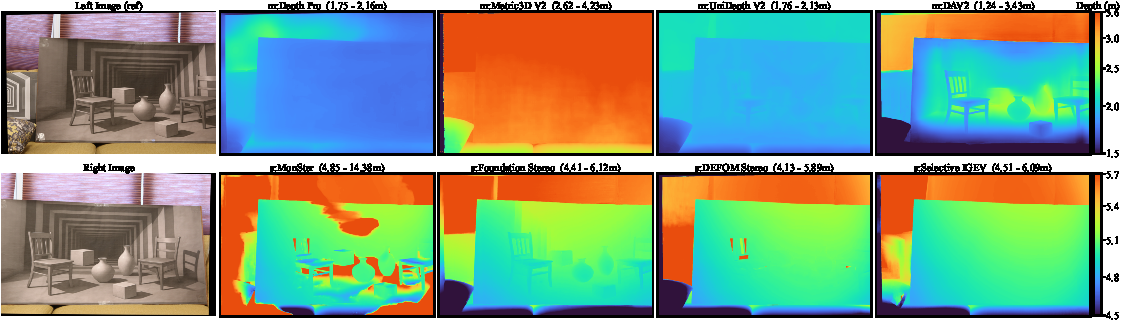
\includegraphics[width=\textwidth]{imgs/illusions_used_S6_16_visualization_frame_0.pdf}\vspace{-10pt}
%     \subcaption{\vspace{-16pt}}
%     \end{subfigure}
%     \begin{subfigure}{\textwidth}
%     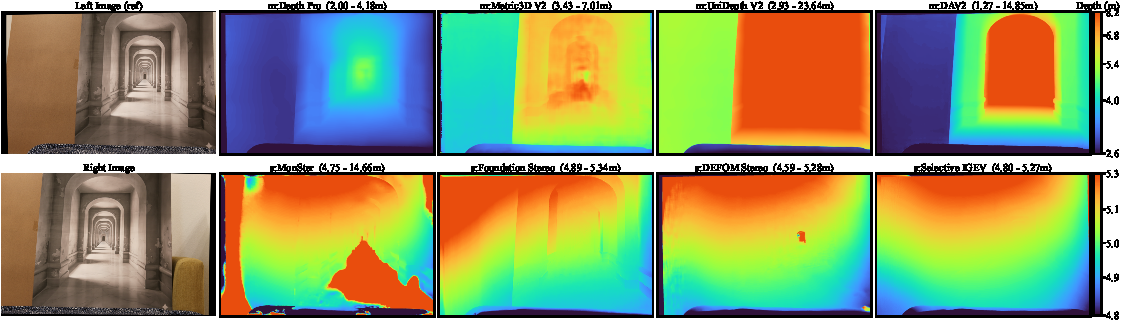
\includegraphics[width=\textwidth]{imgs/illusions_used_S6_10_visualization_frame_0.pdf}\vspace{-10pt}
%     \subcaption{\vspace{-16pt}}
%     \end{subfigure}
%     \begin{subfigure}{\textwidth}
%     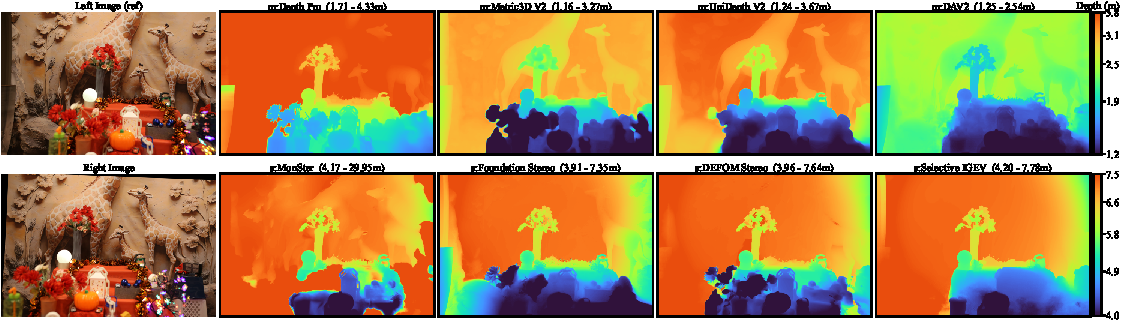
\includegraphics[width=\textwidth]{imgs/S9_f40_img_3901_visualization_frame_0.pdf}\vspace{-8pt}  
%     \end{subfigure}

%     \begin{subfigure}{\textwidth}
%     \begin{minipage}[t]{0.2\textwidth}
%         \centering
%         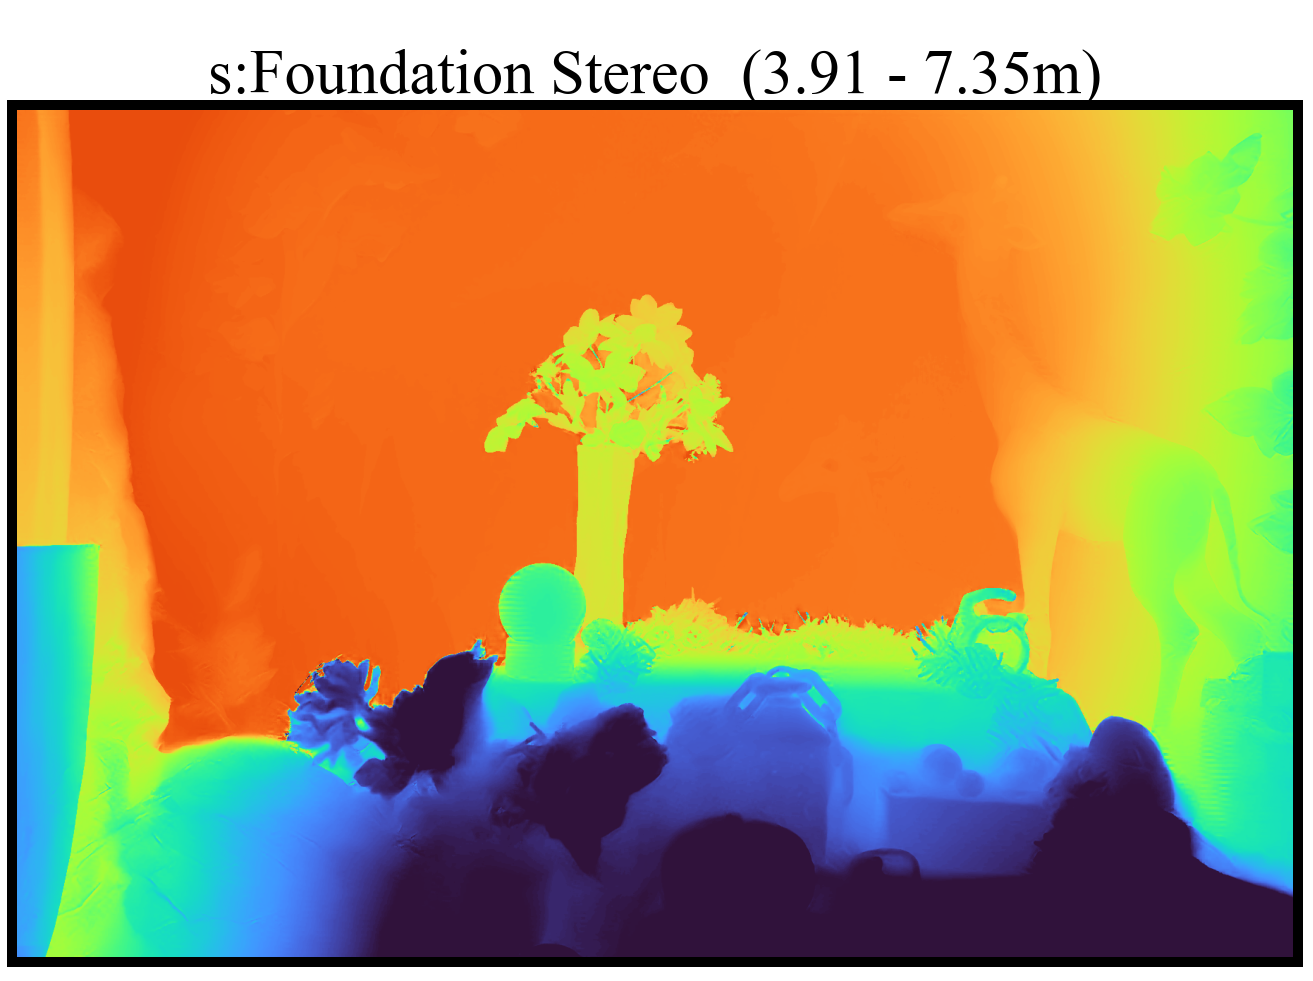
\includegraphics[width=\linewidth,height=0.68\linewidth]{imgs/S9_f40_img_3901_foundation.png}\vspace{-12pt}
%     \end{minipage}%
%     \hfill
%     \begin{minipage}[t]{0.8\textwidth}
%         \centering
%         \includegraphics[width=\linewidth]{imgs/error_maps_7.pdf}\vspace{-12pt}
%     \end{minipage}\vspace{-12pt}   
%     \subcaption{}
%     \end{subfigure}    

%     \caption{SOTA 4 monocular and 4 stereo depth estimation models are evaluated on 3 image pairs with optical illusions. The last row shows four error components for the Foundation Stereo~\cite{foundation} depth map, highlighting errors that are visually subtle but geometrically significant. Gradient error and planarity error $(\times 1e6)$ share a common colormap. All depth maps are produced in the left view. Monocular and stereo models are denoted by m: and s: prefixes respectively; depth ranges show ($5\text{–}95\%$ile).}
%     \label{fig:illusions}
% \end{figure*}






%\subsection{Multi-View Stereo and 3D Reconstruction}\label{subsec:mvs}

%\subsubsection{Classical MVS Limitations}
%We first attempted 3D reconstruction using classical multi-view stereo (MVS) pipelines such as COLMAP~\cite{colmap1,colmap2} and OpenMVS~\cite{openmvs}. While widely used, these geometry-driven approaches exhibit practical limitations on high-resolution indoor scenes. Patch-based stereo relies on photometric consistency and Lambertian reflectance assumptions; therefore reflective, transparent, or glossy materials (e.g., metal, acrylic, glass) introduce severe matching ambiguities and missing regions~\cite{pol_mvs2}. Low-texture or planar surfaces such as walls and cardboard also produce unstable depth estimates due to insufficient discriminative features~\cite{yang_mvs3}.

%From a computational perspective, dense reconstruction is expensive. A full reconstruction using 120 high-resolution views required more than 50\,GB of memory and several hours of runtime on an NVIDIA A100 GPU. Reducing iterations, sampling density, or image resolution accelerates computation but degrades geometric fidelity and depth consistency.

%In our experiments, classical pipelines often produced noisy or incomplete geometry. Smooth or specular surfaces yielded uncertain depth gradients, repeated textures caused mismatches, and thin structures such as wires or plant leaves were frequently unrecoverable. These observations highlight the sensitivity of traditional MVS to reflectance properties, texture availability, and triangulation geometry in realistic indoor scenes.

%\subsubsection{Learning-based Reconstruction}
%To explore modern alternatives, we evaluated a recent learning-based MVS model, MapAnything~\cite{keetha2025mapanything}. Unlike optimization-heavy pipelines such as COLMAP or OpenMVS, this transformer-based architecture predicts globally consistent geometry directly from multi-view images without explicit bundle adjustment or iterative stereo matching.

%The resulting point clouds demonstrate that the model can recover the primary scene structure, including surfaces, background geometry, and major objects, while maintaining spatial continuity across views. Compared to classical MVS, the reconstructions are typically denser and smoother, particularly in regions where traditional stereo struggles (e.g., low-texture or reflective surfaces). However, artifacts remain around thin structures, object boundaries, and specular regions. The model also occasionally interprets planar printed backdrops as volumetric structures, revealing ambiguities between appearance cues and true scene geometry.

%\subsubsection{Evaluation Protocol}
%Our dataset is designed as a diagnostic stress test for multi-view stereo and depth estimation methods rather than a benchmark with absolute ground truth. We therefore do not treat COLMAP reconstructions as reference geometry. Instead, methods are analyzed through downstream tasks such as depth-of-field rendering and defocus deblurring, which expose geometric inconsistencies. This protocol emphasizes identifying systematic failure modes rather than ranking methods against potentially biased reconstructions.

%\subsection{Neural 3D Representations (NeRF, GS)}\label{subsec:use_gs}

%Although 3D reconstruction is not the primary motivation of this work, the dataset can also support neural scene reconstruction approaches such as NeRF-style radiance fields and Gaussian Splatting (GS). The calibrated multi-view captures with varying focal lengths and apertures provide the geometric consistency and photometric diversity required for training and evaluating neural 3D representations.

%Both reconstructions produced using a learning-based MVS method and Gaussian Splatting via Splatter3R~\cite{smart2024splatt3r} recover coherent global structure but exhibit characteristic artifacts, including floating geometry near thin structures and inconsistencies where optical appearance cues conflict with true 3D layout. These observations suggest that MODEST can serve as a challenging dataset for evaluating next-generation neural reconstruction methods, particularly under complex indoor scenes and aperture-dependent image formation.

%Together, these evaluations demonstrate that MODEST exposes consistent failure modes in existing models that synthetic and low-resolution benchmarks do not, motivating the need for high-resolution, real-optics datasets in future training and evaluation pipelines






% \begin{figure}[t]
% \centering
% \includegraphics[width=0.49\linewidth,height=3.2cm]{imgs/MVS-demo.pdf}
% \hfill
% \includegraphics[width=0.49\linewidth,height=3.2cm]{imgs/GS2.pdf}

% \vspace{-3pt}
% \caption{Example 3D reconstructions on MODEST. 
% Left: learning-based multi-view stereo (MapAnything~\cite{keetha2025mapanything}). 
% Right: Gaussian Splatting using Splatter3R~\cite{smart2024splatt3r}. 
% These results illustrate that the dataset can also support neural 3D reconstruction, although this is not the main focus of the paper.}
% \label{fig:3d_scene}
% \vspace{-8pt}
% \end{figure}
\section{Conclusion}\label{sec:conclusion}

% In this work, we introduced the first high-resolution, controlled-optics, balanced, real-world stereo dataset designed for real-world shallow depth-of-field rendering, deblurring and other applications. With optical and geometric errors and visual evidence, we demonstrated that existing DoF rendering and deblurring models degrade substantially under real lens optics, and that classical and learning-based 3D reconstruction pipelines exhibit characteristic as challenging indoor scenes. We highlight the need of datasets such as MODEST to assess quality of these models under real-world camera optics variations and challenging optical illusions. To support future research, we release the complete dataset, illustrations and visuals, processing and evaluation tools for purely non-commercial, academic research purposes. With 20000 high-fidelity images and real camera optics, we hope this dataset serves as a catalyst for advancing shallow depth-of-field, depth estimation and related technologies towards more robust real-world performance.

In this work, we introduced the first high-resolution, controlled-optics, balanced, real-world stereo dataset designed for real-world shallow depth-of-field (DoF) rendering and defocus deblurring. With quantitative and visual evidence, we demonstrated that existing DoF rendering and deblurring models degrade substantially under real lens optics as challenging indoor scenes. We highlight the need for datasets such as MODEST to assess the quality of these models under real-world camera optics variations for DoF and defocus deblurring tasks. To support future research, we release the complete dataset, illustrations and visuals, processing and evaluation tools for purely non-commercial, academic research purposes. With 20000 high-fidelity images and real camera optics, we hope this dataset serves as a catalyst for advancing shallow depth-of-field, depth estimation, and related technologies towards more robust real-world performance.


\clearpage  % TODO FINAL: This \clearpage needs to be removed from both review and camera-ready versions.
% ---- Bibliography ----
%
% BibTeX users should specify bibliography style 'splncs04'.
% References will then be sorted and formatted in the correct style.
%
\bibliographystyle{splncs04}
\bibliography{main}
\end{document}